\lab{Applications}{Job Search Model}{Job Search Model}

\section*{Discrete Choice (Threshold) Problems}\label{SecDiscrChoice}

One powerful application of dynamic programming is
to models that have both continuous and discrete state variables. These models are sometimes referred to as
discrete choice problems or optimal stopping problems.  Examples include models of employment that involve both
the choice of whether to work and how much to work, models of firm entry and exit that involve the choice of both
whether to produce and how much to produce, and models of marriage that involve the choice of whether to date
(get married or keep dating) and how much to date.
This application illustrates the versatility of dynamic programming as a dynamic solution method

In this lab, we follow a simple version of a standard job search model.
Assume that workers live infinitely long. 
We will split a worker's life into discrete time periods, and in each period the worker is either
employed or unemployed, and receives a job offer. The worker must make a choice between discrete actions
(such as accepting or rejecting a job offer), with the goal of maximizing some utility function (hence,
this is a \emph{discrete choice} problem).

We can state this problem in terms of dynamic programming by defining an appropriate value function.
Let the value of entering a period with most recent wage $w$,
current job offer wage $w'$, and employment status $s$ be given by the following value function,
\begin{equation}\label{EqV}
   V(w,w',s) = \begin{cases}
                  V^E(w)    \quad&\text{if}\quad s = E \\
                  V^U(w,w') \quad&\text{if}\quad s = U \\
               \end{cases}
\end{equation}
where employment status is a binary variable $s\in\{E,U\}$ ($E$ indicates ``employed" and $U$ indicates ``unemployed");
a person can be either employed or unemployed.

As in the cake eating problem, the value function is calculated as the sum of some reward (based on the 
current state) and the discounted value of entering the next period in some particular state.
The reward function, denoted (as usual) by $u$, gives the utility of spending available funds. 
Assuming that a worker receives some wage $x$ in a given period and spends all available money in the period,
the utility of consumption is given by
\[
u(x).
\]
Calculating the value for the next period depends on the employment status in the current period, so we address
this separately for each case.

Let us first consider the case where the individual is unemployed ($s = U$). As is customary, let $s'$ denote the
employment status of the worker in the next period.
In this unemployed state, the worker receives unemployment benefits equal to a fraction of her most recent wage,
i.e. $\alpha w$, where $\alpha \in (0, 1)$. 
Hence, the utility of consumption in the current unemployed state is given by
\[
u(\alpha w).
\]

The worker also receives one wage offer ($w'$) per period, and will obtain
this wage in the next period provided that he chooses to accept employment, i.e. provided $s' = E$.
The worker must decide whether to accept the current wage offer $w'$ or to remain unemployed in the next period, 
i.e. he must decide on the value of $s'$. How
does he make this choice? He must weigh the value of entering the next period as an employed worker with wage
$w'$ (given by $V^E(w')$) versus the value of entering the next period as an unemployed worker with
previous wage $w$ and unknown wage offer $w''$ (given by $V^U(w,w'')$). Because the worker cannot know
what the future wage offer $w''$ will be, it is treated as a random variable with a particular probability
distribution. Hence, the worker must actually compute the \emph{expected} value of entering the next
period unemployed. This term is simply
\[
\mathbb{E}_{w''}V^U(w,w''),
\]
where $\mathbb{E}_{w''}$ denotes the expectation operator with respect to the probability distribution of future
wage offers $w''$.
To sum up, the worker chooses to accept the wage offer $w'$ or remain unemployed in the next period based on
which option gives the greater expected value, and the value of this decision is given by
\[
\max\Bigl\{V^E(w'), \,\, \mathbb{E}_{w''}V^U(w,w'')\Bigr\}.
\]

The overall value of the current unemployed state with previous wage $w$ and current wage offer $w'$ is
just the utility of consumption plus the the discounted value of the next period, i.e.
\begin{equation}\label{EqVu}
V^U(w,w') = u(\alpha w) + \beta \max\Bigl\{V^E(w'), \,\, \mathbb{E}_{w''}V^U(w,w'')\Bigr\},
\end{equation}
where $\beta$ is the discount factor.

Now we turn to the case where the job status is employed ($s = E$).
In this case, the worker receives a wage $w$ in the current period, and so the utility of consumption is 
just
\[
u(w).
\]
In the next period, the worker will have most recent wage $w$, she will receive wage offer $w''$, and will 
have employment status $s'$. As in the unemployed case, $w''$ is unknown and treated as a random variable.
Unlike the unemployed case, however, the worker's future employment status $s'$ is not under her control, 
but rather is also a random variable. The reason for this is that the worker will remain employed 
until she loses the job, a random event that occurs with some fixed probability in each time period.
Hence, we must calculate the expected value of the next period with respect to both $w''$ and $s'$. 
We may write the entire value function for the employed case as
\begin{equation}\label{EqVe1}
   V^E(w) = u(w) + \beta \mathbb{E}_{w'',s'}V(w,w'',s').
\end{equation}

To calculate the expectation term, we need to know the joint probability distribution over $w''$ and $s'$.
This can be characterized in the following way.
We assume that $s'$ and $w''$ are independent. Hence, we can split the joint expectation
operator into the composition of the two individual expectation operators:
\[
\mathbb{E}_{w'',s'} = \mathbb{E}_{w''}\mathbb{E}_{s'}.
\]
Let $\gamma$ represent the probability that an employed worker becomes unemployed in the next period,
so that $1-\gamma$ is the probability of remaining employed in the next period.
If the worker stays employed in the next period ($s' = E$), then next period's wage equals the current
period's wage, and the term inside the expectation is
\[
V(w,w'',E) = V^E(w).
\]
We then have
\begin{align*}
\mathbb{E}_{s'}V(w,w'',s') &= (1-\gamma)V(w,w'',E) + \gamma V(w,w'',U)\\
&= (1-\gamma)V^E(w) + \gamma V^U(w,w'').
\end{align*}
Notice that the term $(1-\gamma)V^E(w)$ is constant with respect to $w''$. Then
\begin{align*}
\mathbb{E}_{w''}\mathbb{E}_{s'}V(w,w'',s') &= \mathbb{E}_{w''}\left[(1-\gamma)V^E(w) + \gamma V^U(w,w'')\right]\\
&= \mathbb{E}_{w''}(1-\gamma)V^E(w) + \mathbb{E}_{w''}\gamma V^U(w,w'')\\
&= (1-\gamma)V^E(w) + \gamma \mathbb{E}_{w''}V^U(w,w'').
\end{align*}
Hence, we can rewrite \eqref{EqVe1} as follows:
\begin{equation}\label{EqVe2}
   V^E(w) = u(w) + \beta \Bigl[(1-\gamma)V^E(w) + \gamma \mathbb{E}_{w''}V^U(w,w'')\Bigr].
\end{equation}

We have now completely described the value function. What about the policy function?
The policy function for the unemployed worker gives his decision on whether to accept the job $s'=E$ 
or to reject the job $s'= U$. 
This will be a function of both the most recent wage $w$ and the current wage offer $w'$.
The employment status $s'$ in the next period is determined by the policy function $\psi$:
\[
s' = \psi(w,w').
\]

These discrete choice problems are often called threshold 
problems because the policy choice depends on whether the state variable is greater than or less than 
some threshold level. That is, an unemployed worker will accept a job if and only if the offer wage is 
above some set amount that depends on the most recent wage $w$. In the labor search model, 
the threshold level is called the ``reservation wage'' $w_R'$. The reservation wage $w_R'$ is defined as 
the wage offer such that the worker is indifferent between accepting the job $s' = E$ and 
staying unemployed $s' = U$. Hence, this reservation wage satisfies the equation
\begin{equation}\label{EqWR}
   V^E(w_R') = E_{w''}\left[V^U(w,w'')\right].
\end{equation}
The policy function will then take the form of accepting the job if $w' \geq w_R'$ or 
rejecting the job offer and remaining unemployed if $w' < w_R'$:
\begin{equation}\label{EqSprime}
   s' = \psi(w,w') = \begin{cases}
                      E \quad\text{if}\quad w' \geq w_R' \\
                      U \quad\text{if}\quad w' < w_R'.
                   \end{cases}
\end{equation}
Figure \ref{fig:disc_policy} shows an example of the discrete policy function.

\begin{figure}
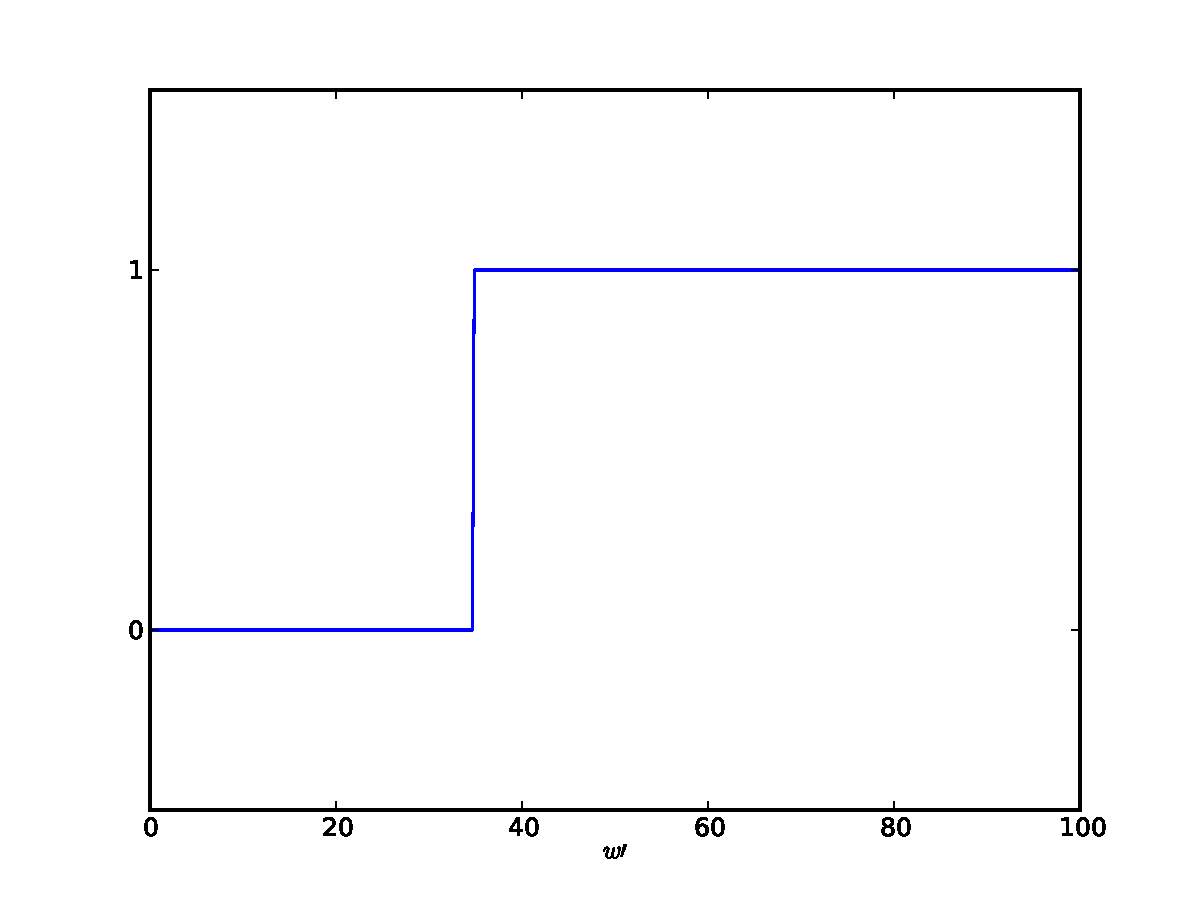
\includegraphics[width=\textwidth]{disc_policy.pdf}
\caption{Here is the policy function for fixed $w = 50$.  Numerically we let 0 represent unemployment, $U$, 
and 1 represent employment, $E$.  Thus we see that an individual will choose to take a new job, given 
their old wage was 50, at a wage of roughly 35.  Thus for a previous wage of 50, we say the reservation wage is 35.}
\label{fig:disc_policy}
\end{figure}

In summary, the labor search discrete choice problem is characterized by the value functions \eqref{EqV}, \eqref{EqVu},
and \eqref{EqVe2}, the reservation wage \eqref{EqWR}, and the policy function \eqref{EqSprime}. Because wage offers
are distributed according to some given probability distribution (denote the cdf by $F(w')$),
and because the policy function takes the form of \eqref{EqSprime},
the probability that the unemployed worker receives a wage offer that he will reject is $F(w_R')$ and the probability
that he receives a wage offer that he will accept is $1 - F(w_R')$. Just like the continuous choice cake eating
problems, this problem can be solved by value function, policy function, or modified policy function iteration.

The value function iteration solution method for the equilibrium in the labor search problem is analogous to the 
value function iteration from the previous labs. The only difference is that two value functions ($V^E$ and $V^U$) 
must converge to a fixed point in this problem instead of just one value function converging in the previous problems.  
Although there are two value functions to consider, there is only one policy function since decisions are only made 
in the unemployed state.  Thus, there is only one policy function on which to iterate in the case of policy or modified 
policy iteration.

Assume that the probability of becoming unemployed in a given period is $\gamma = 0.10$, the fraction of wages paid 
in unemployment benefits is $\alpha = 0.5$, and the discount factor is $\beta = 0.9$. Assume that the log of wage 
offers are distributed normally.  We then say that offers are distributed lognormally and write 
\[
w'\sim \text{LogN}(\mu,\sigma).
\]  
We let $m=20$ be the mean wage, $v=400$ be the variance of the wage.  
Often lognormal distributions are reported with the mean and variance of $\log(w')$ which is distributed normally, 
but for simplicity you will not have to deal with that here. This is a convenient choice for the distribution of 
wage offers.  Among other things, it guarantees that wage offers will be positive.  Denote the cdf of the 
lognormal distribution as $F(w')$ and the pdf of the distribution as $f(w')$.

\begin{problem}
Solve the job search problem by carrying out the following steps.
\begin{enumerate}

   \item Approximate the support of $w\in(0,\infty)$ by generating a column vector of possible values for $w$. 
   Let the maximum value be $w_{max} = 100$, let the minimum value be $w_{min} = 0$, and let the number of 
   equally spaced points in the vector be $N = 500$. Let the wage of a job offer in any period be lognormally 
   distributed with mean job offer of $m=20$ and variance $v =200$.  Generate the discrete approximation of the 
   lognormal probability density function $f(w')$ using the function defined in discretelognorm.py which is 
   provided.  As arguments, it takes the points where the approximation is needed (w), along with the mean and 
   variance so that it can be called as

\begin{lstlisting}
f = discretelognorm(w,m,v)
\end{lstlisting}

    Then the $n$th entry of $f$ represents the probability that the job offer in the next period equals the 
    $n$th entry of $w$, $\text{Pr}(w' = w_n)$.

   \item Solve for the equilibrium optimal policy function $s' = \psi(w,w')$ by value function iteration.  
   In this case we iterate on both value functions $V^E$ and $V^U$ each time through the loop.  In order to 
   compute the expected value of $V^U$, just matrix multiply $V^U$ and $f$. Remember, the policy function 
   $\psi(w,w')$ gives the choice of whether to accept the job offer if unemployed with a given previous wage 
   and current job offer.  Thus it will be a vector of length $N$ of zeros and ones.  Again, use a tolerance 
   level of $10^{-9}$ and require that both value functions must converge (compute a delta for each and iterate 
   until both are less than $10^{-9}$).

   \item Compute the reservation wage $w_R'$ as a function of the current wage $w$.  The reservation wage is the 
   value of $w$ where the policy function changes from zeros to ones (the optimal choice changes from remaining 
   unemployed to accepting the job offer).  If psi is an $N\times N$ matrix representing the policy function, the 
   reservation wage wr could be computed as follows
   \begin{lstlisting}
    wr_ind = sp.argmin(sp.diff(psi), axis = 1)
    wr = w[wr_ind]
   \end{lstlisting}
	where the rows of psi correspond to values of $w$ and the columns correspond to values of $w'$.

   \item Plot the equilibrium reservation wage $w_R'$ of the converged problem as a function of the current 
   wage $w$ with the current wage on the $x$-axis and the reservation wage $w_R'$ on the $y$-axis. This is 
   the most common way to plot discrete choice policy functions. The reservation wage represents the wage 
   that makes the unemployed worker indifferent between taking a job offer and rejecting it. So any wage 
   above the reservation wage line represents $s' = E$ and any wage below the reservation wage line represents 
   $s' = U$.

\end{enumerate}
\end{problem}

In the previous problem, it was necessary to iterate on two value functions.  Consequently the convergence is relatively slow.  Thus the gains by using modified policy function iteration are considerable.

\begin{problem}
Solve the same problem, this time using modified policy function iteration with $m=15$ value function iterations within each policy iteration.  Roughly, you can structure your code as follows:

\begin{enumerate}
	\item Initialize $w$,$u(\alpha w)$, $f$, $\gamma$, and $\beta$.  This should be the same as the previous problem.
	
	\item	Initialize $V^E$, $V^U$, and $E[V^U]$ to zeros.  Then begin the while loop.
	
	\item Inside the while loop update the policy function.  It is determined as
	\begin{equation}
		\psi (w,w') = \text{argmax} \left\{ V^E(w'), E_{w''}[V^U(w,w'')]\right\}
	\end{equation}
	
	\item Begin a for loop to iterate on the value functions.  Unlike in the previous algorithms lab, there is no $Q$ matrix in this case.  Given the previous iteration's value functions, updating $V^E$ should be simple because it does not depend directly on the policy function.
	
	To iterate on $V^U$, we need to compute $V^U$ given the current policy.  The policy determines the maximization in equation \eqref{EqVu}.  One way to compute the max is to use $\psi$ as a mask.  $V^U$ could be computed as follows:
	
\begin{lstlisting}
arg1 = sp.repeat(sp.transpose(VE),N,0)*psiprime
arg2 = sp.repeat(EVU,N,1)*(1-psiprime)
arg = arg1+arg2
VUprime = alpha_util_grid + beta*arg
\end{lstlisting}	

	where the ordering is such that $1$ corresponds to the state $E$ and $0$ corresponds to the state $U$.
	
	\item Compute the $\delta$'s.
	
	\item After the while loop you should compute the reservation wage and plot it.
\end{enumerate}
\end{problem}

\begin{problem}
How many iterations did value function iteration take?
How many iterations did modified policy function iteration take?
Which was faster?
\end{problem} 